% !TEX root = main.tex

We present the results of the LCA analysis in relation to the 1) embodied GWP, 2) a calculation of the emission factor, 3) sensitivity of the LCA to design and location, and 4) a comparison to other PV technologies.

\subsection{LCA of the Adaptive Solar Facade Manufacture}

A breakdown of the embodied global warming potential (GWP) can be found in Figure  \ref{fig:embodied}. The largest embodied GWP contribution in the ASF comes from the solar panels, the electronics and the supporting structure.

\begin{figure}[H]
\begin{center}
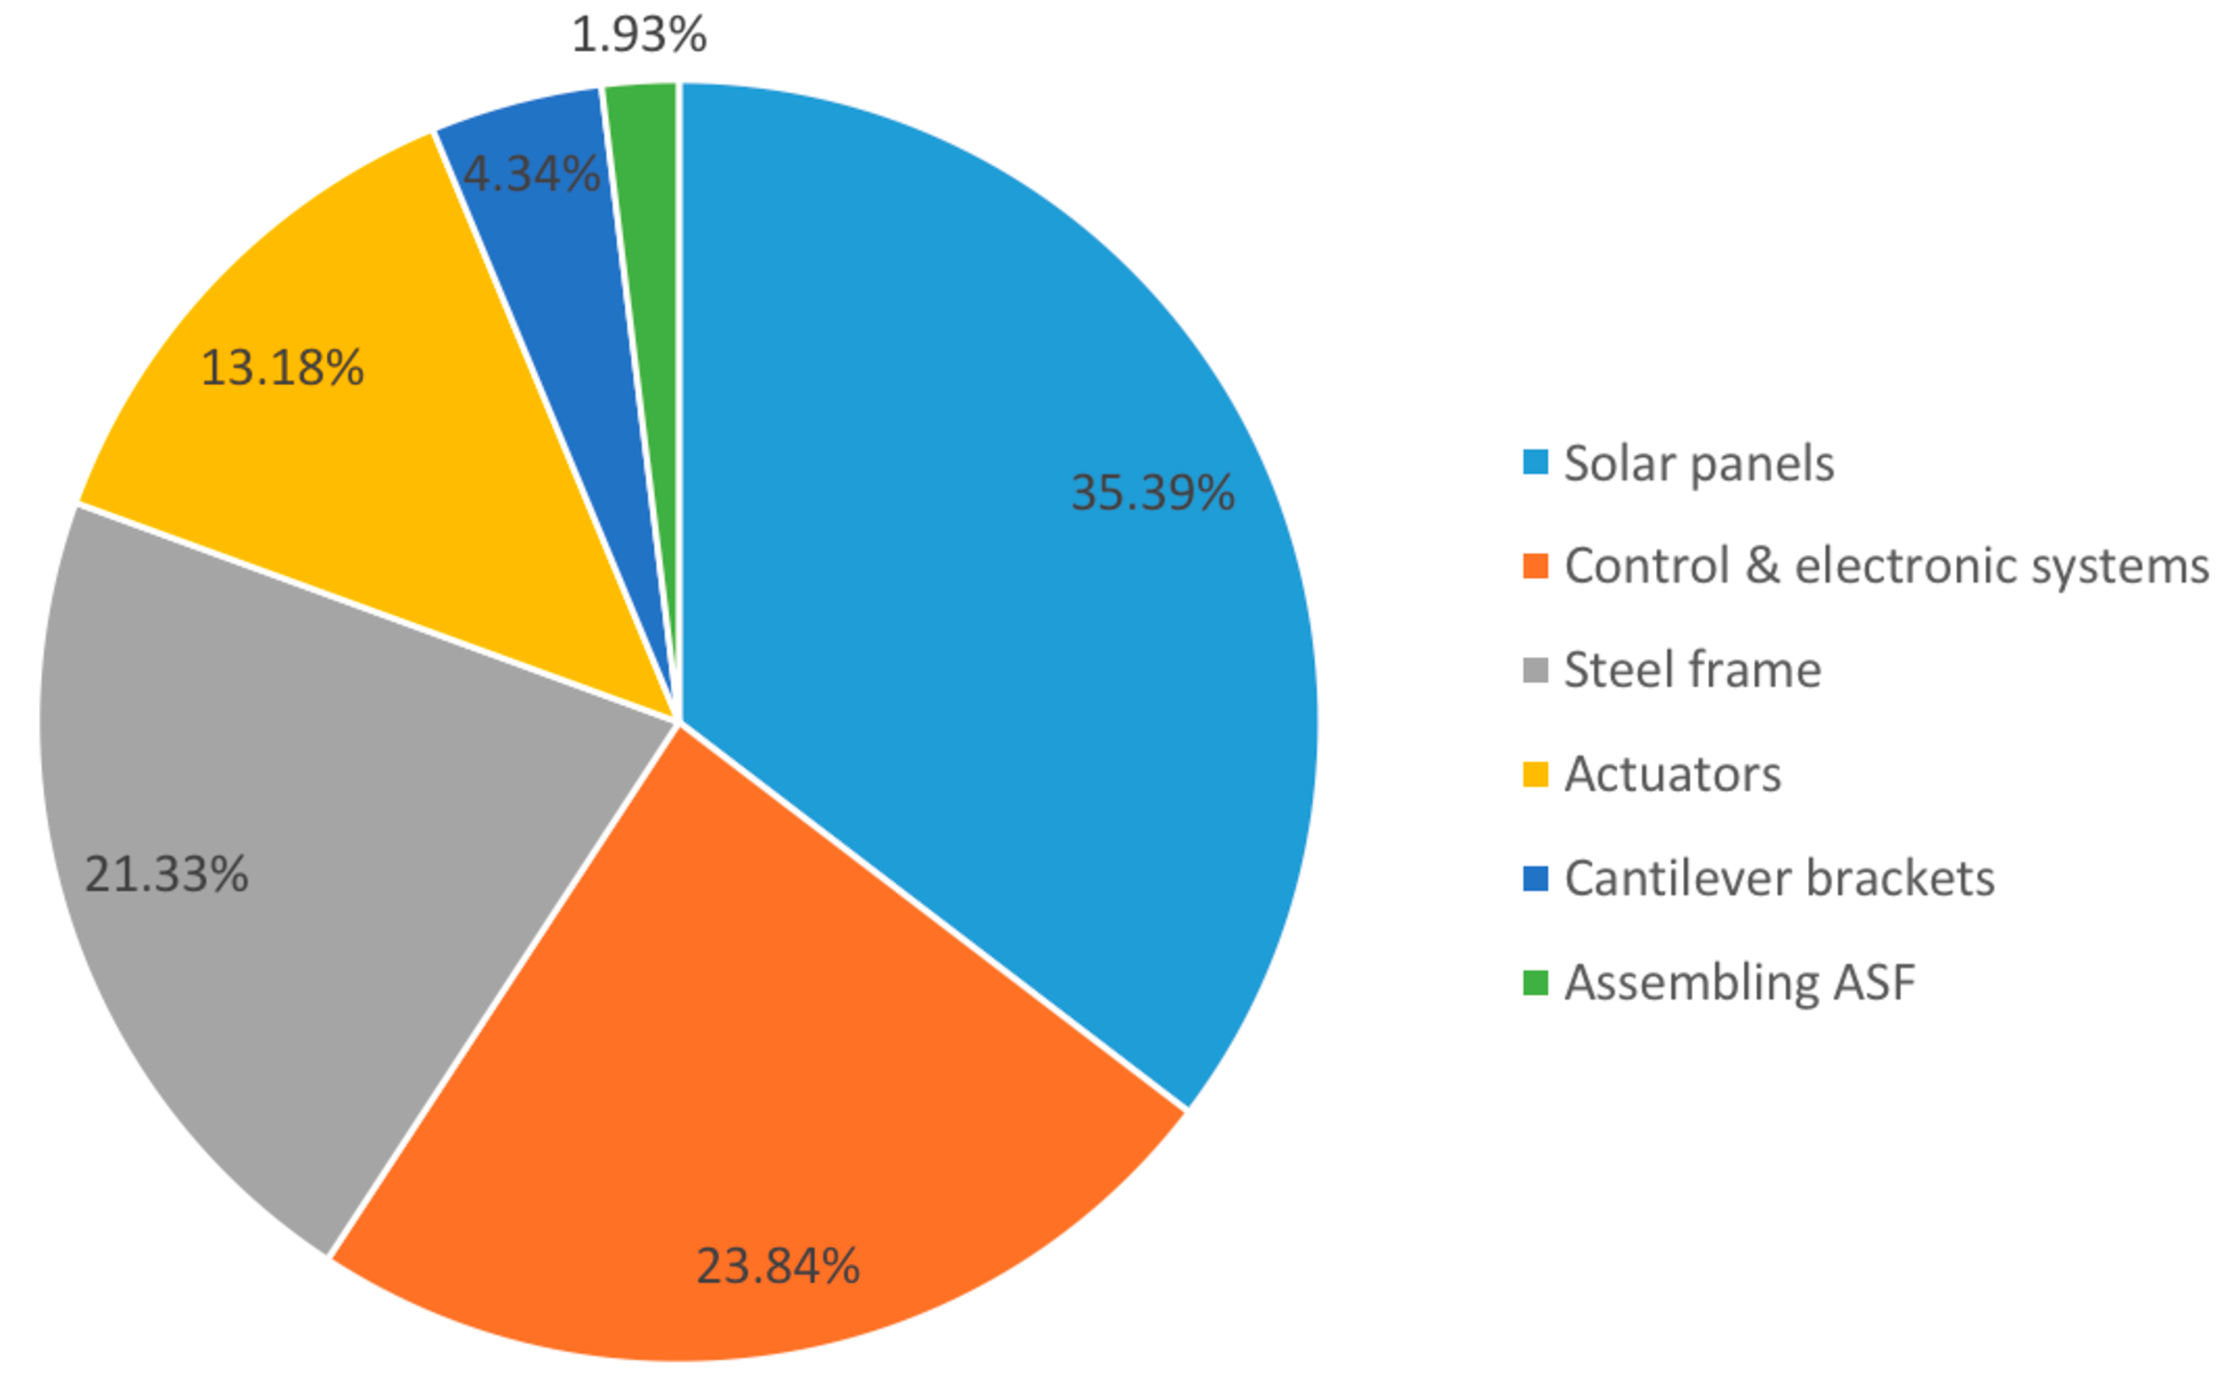
\includegraphics[width=10cm, trim= 0cm 0cm 0cm 0cm,clip]{pieembodied}
\caption{Breakdown of greenhouse gas emissions due to material production. The total is GWP is 2676 kg CO$_{2-eq}$}
\label{fig:embodied}
\end{center}
\end{figure}

\subsection{Calculation of Emission Factor}
The combined GWP of main inputs to the ASF, previously described in Figure \ref{fig:BOS}, can be built up using a waterfall chart as shown in Figure \ref{fig:waterfall}. 

This gives us a total GWP of -6229.6 kg CO$_{2-eq}$. We calculate a total electricity production of 518kWh per year, resulting in an emission factor of -601.1 gCO$_{2-eq}$/kWh.

\begin{figure}[H]
\begin{center}
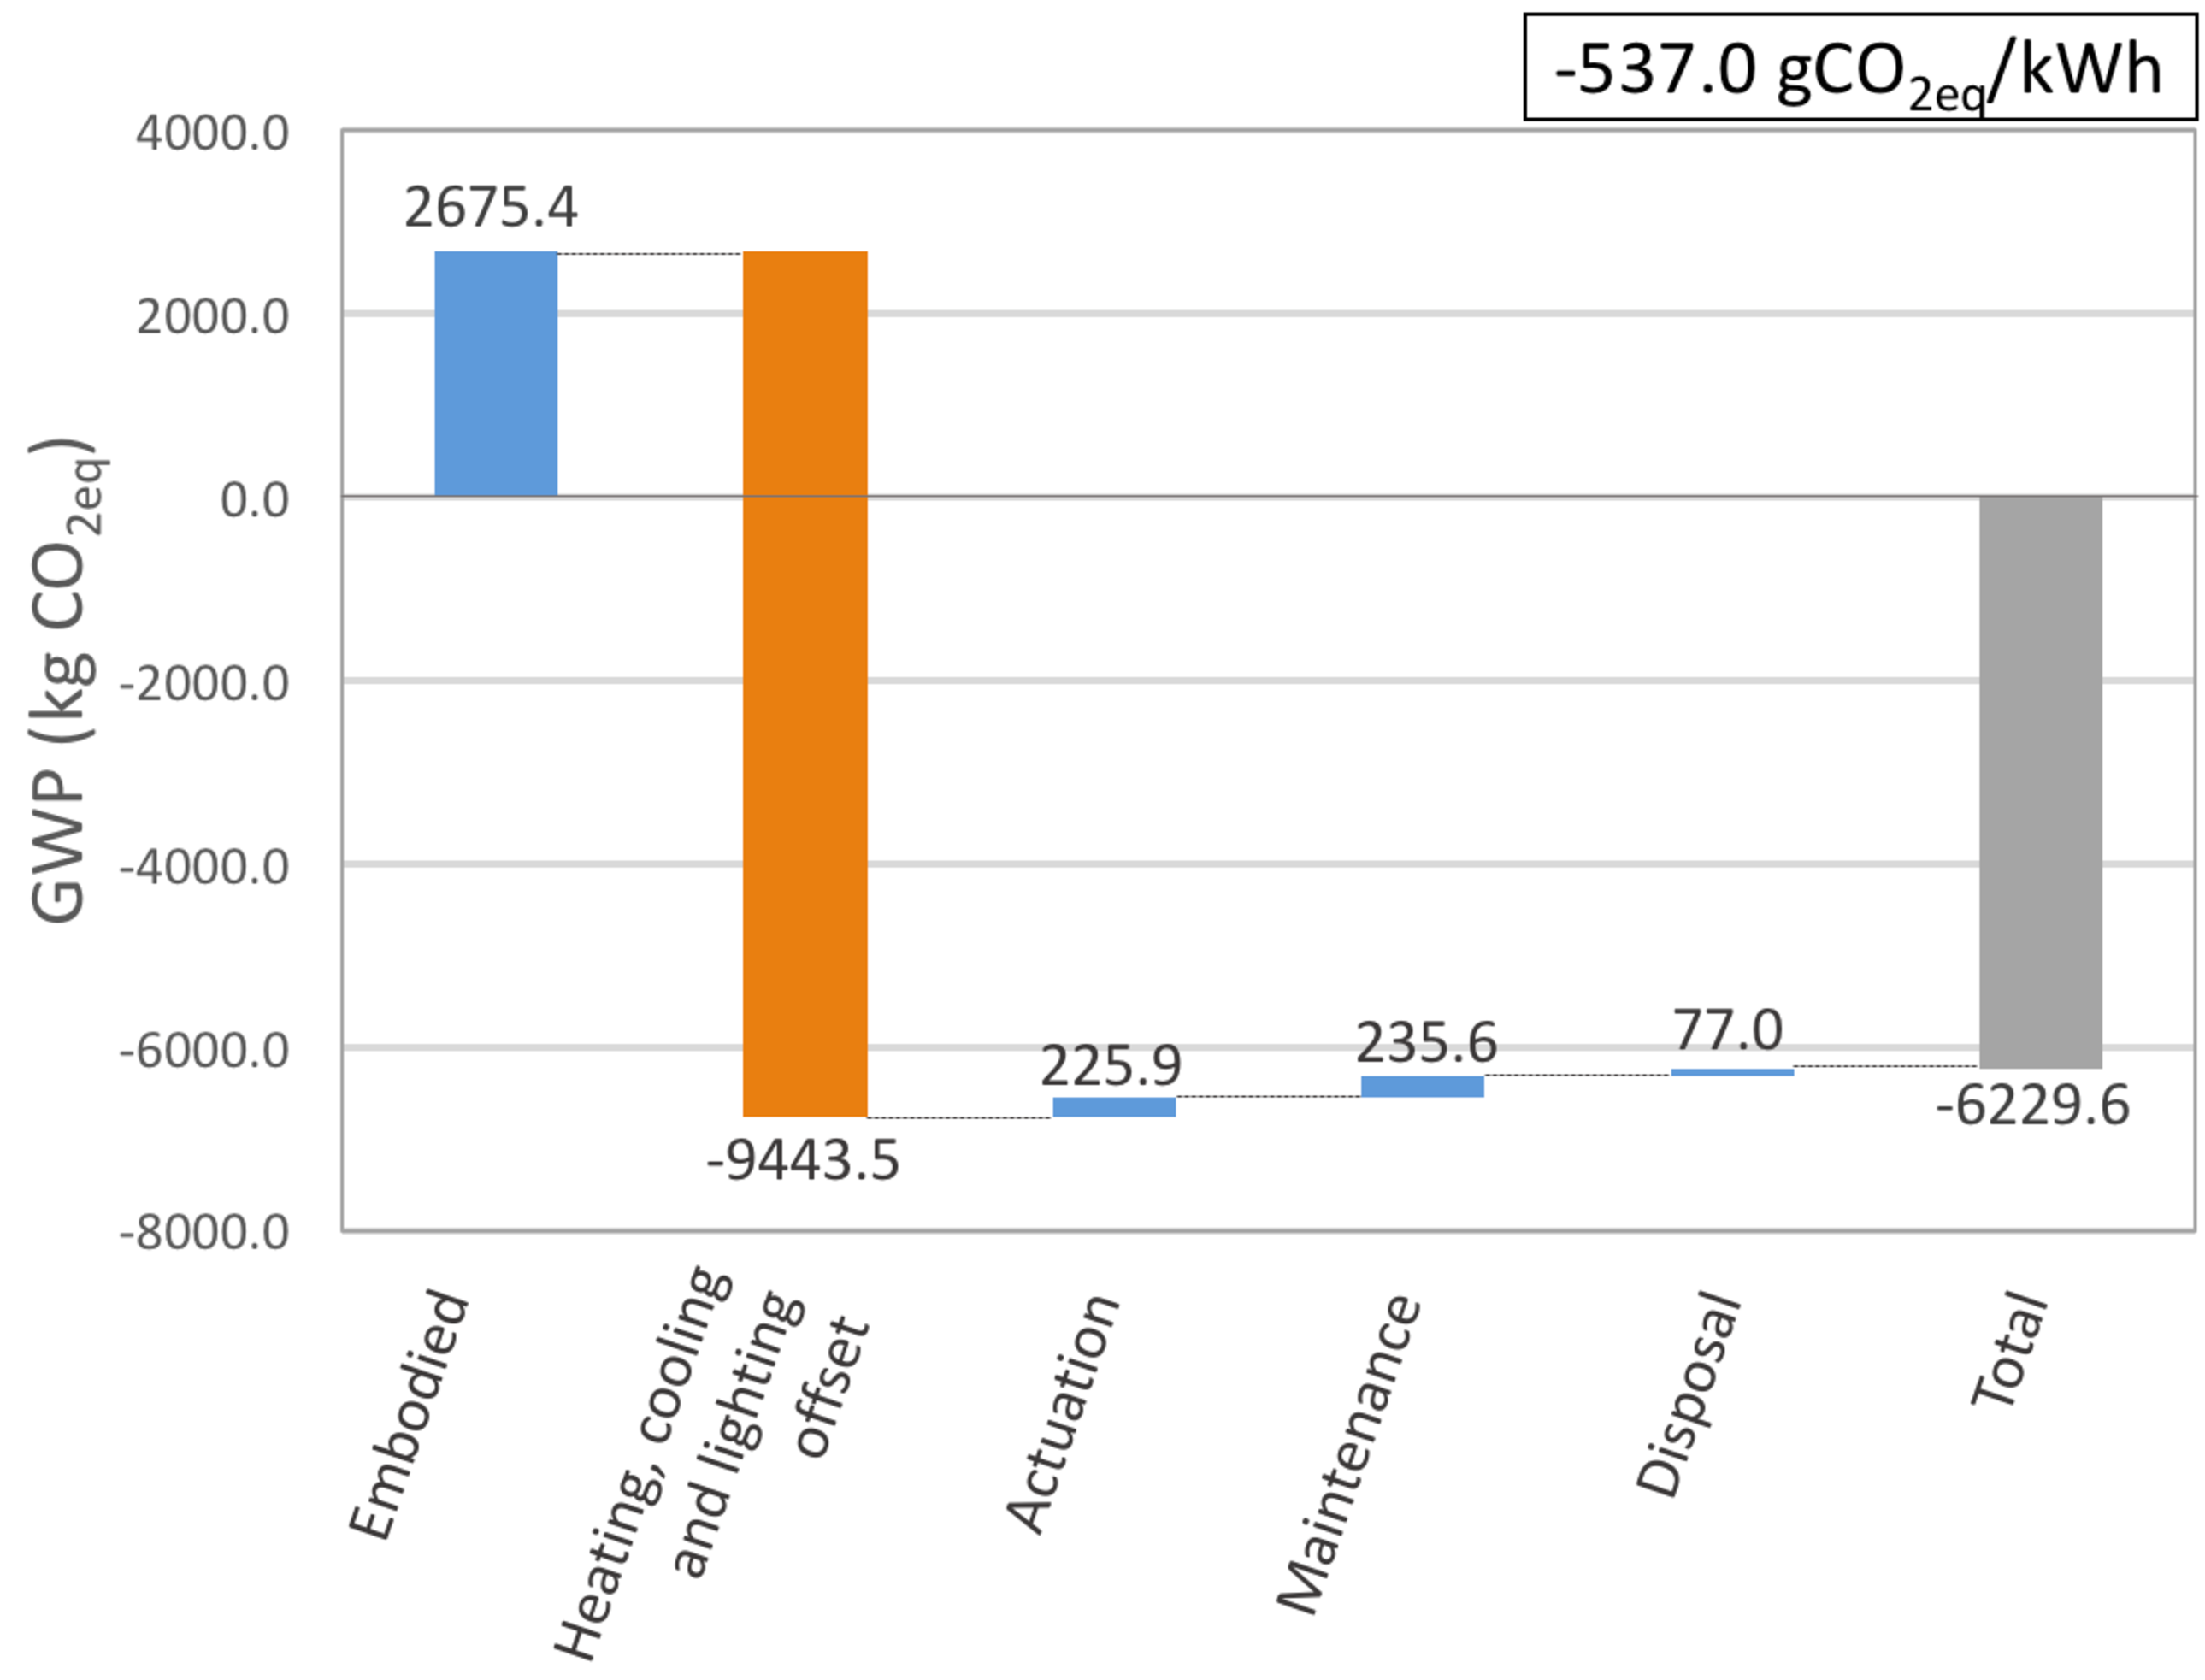
\includegraphics[width=12cm, trim= 0cm 0cm 0cm 0cm,clip]{waterfall}
\caption{Waterfall diagram of GWP of the ASF. The far left bar details the embodied carbon emissions. The second bar details the emission reduction of the building through adaptive shading. The third, fourth and fifth bar shows the effect of dynamic actuation, maintenance, and disposal respectively. This leaves us with a final emissions value (grey bar). When we apply this value to Equation \ref{eq:EF}, we obtain an emission factor per kWh of -601.1 gCO$_2$-eq./kWh. Note that the waterfall chart itself doesn't show PV electricity generation. This is taken into account in the emission factor.}

\label{fig:waterfall}
\end{center}
\end{figure}

% \subsection{Global Distribution of GWP and Terrestrial Acidification}


% \textcolor{magenta}{\textit{Sorry that I keep coming back to this. How is this relevant to the overall scope of the paper? You should probably pick it up again in the Conclusion or Discussion. Furthermore you should describe (e.g. in the Methodology) how the regionalized LCA was performed.\\
% As I said - these figures are likely to be wrong. If one of the reviewers is an LCA crack, he / she might attack this.}}

% The global distribution of embodied GWP emissions is focused in Europe, specifically Germany and Switzerland as most of the manufacturing is done in this region. It can be see however that emissions occur globally due the sourcing of primary materials from many locations around the world. Terrestrial acidification however is more interesting as it has a local impact compared to carbon emissions. It is interesting to note that China carries the greatest burden of terrestrial acidification from the ASF production.
 
% \begin{figure}[H]
% \begin{center}
% 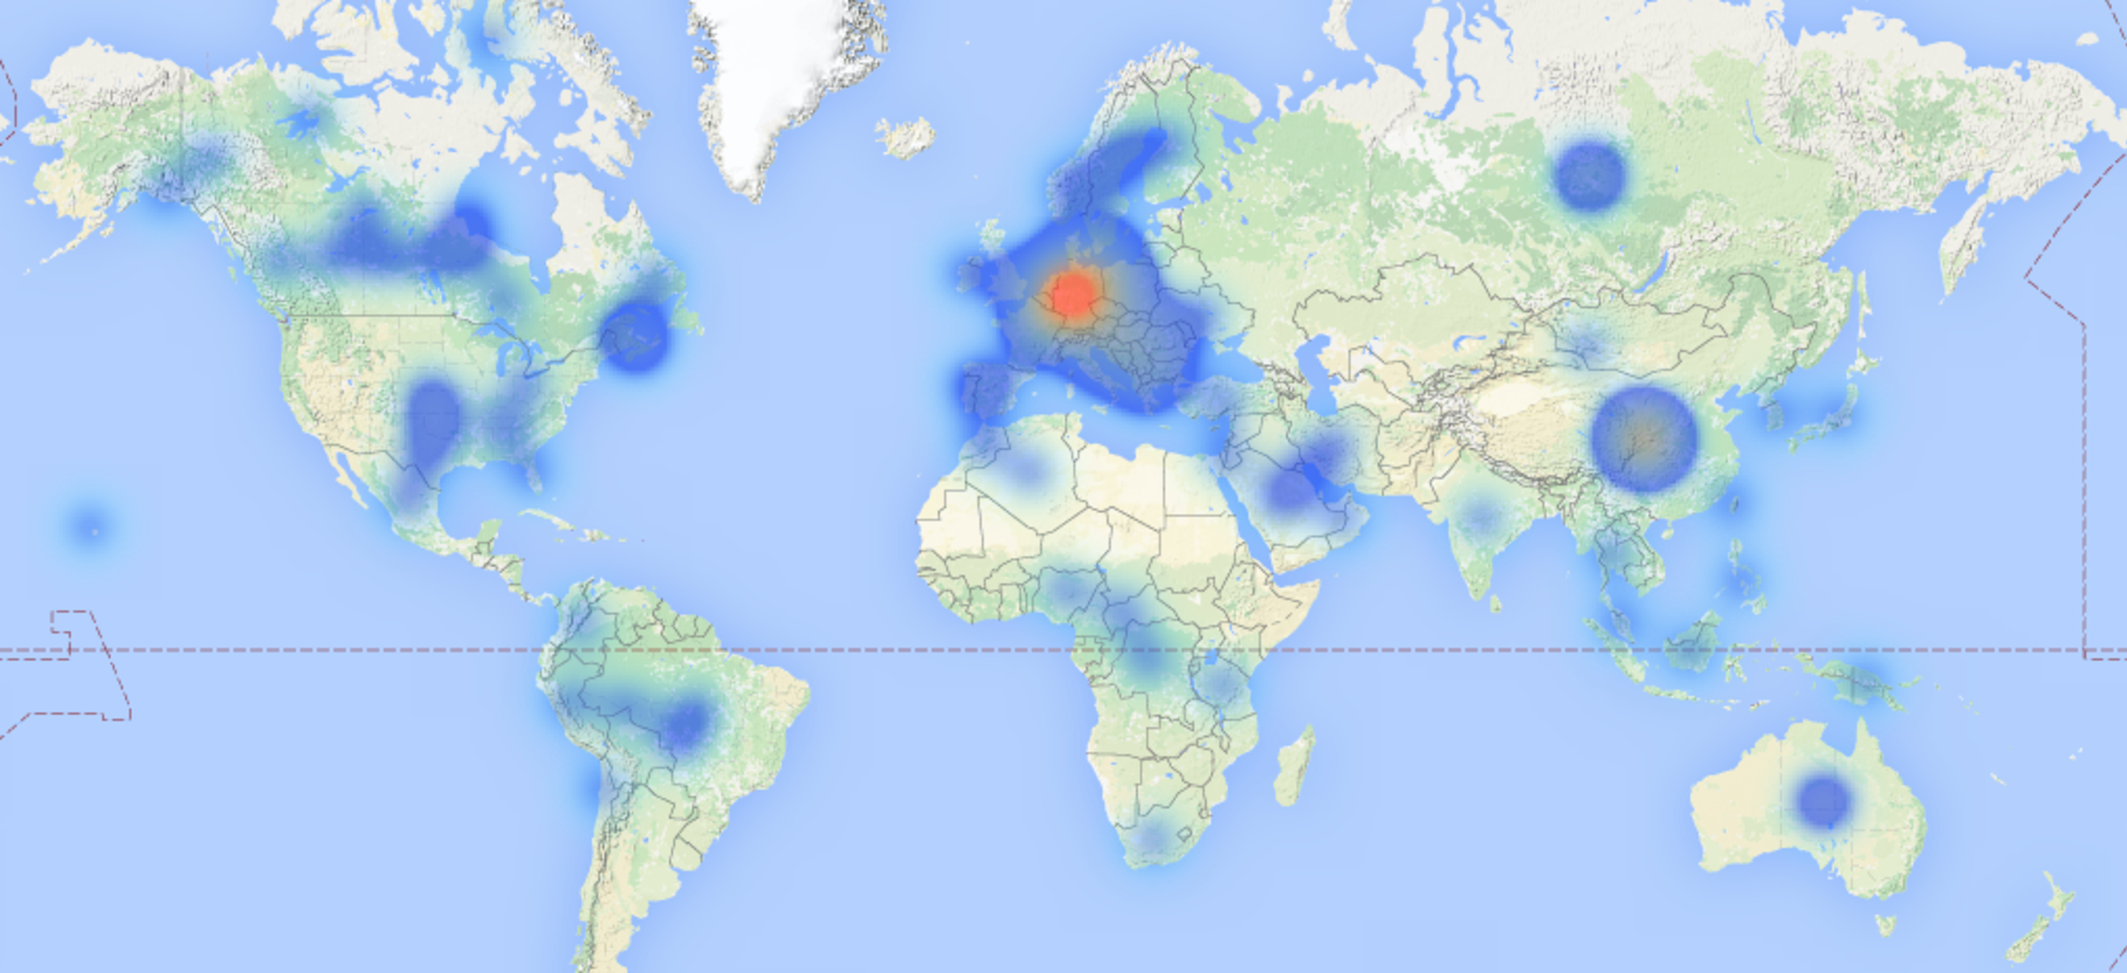
\includegraphics[width=10cm, trim= 0cm 0cm 0cm 0cm,clip]{mapGWP.pdf}
% \caption{Global distribution of embodied GWP emissions}
% \label{fig:mapGWP}
% \end{center}
% \end{figure}

% \begin{figure}[H]
% \begin{center}
% 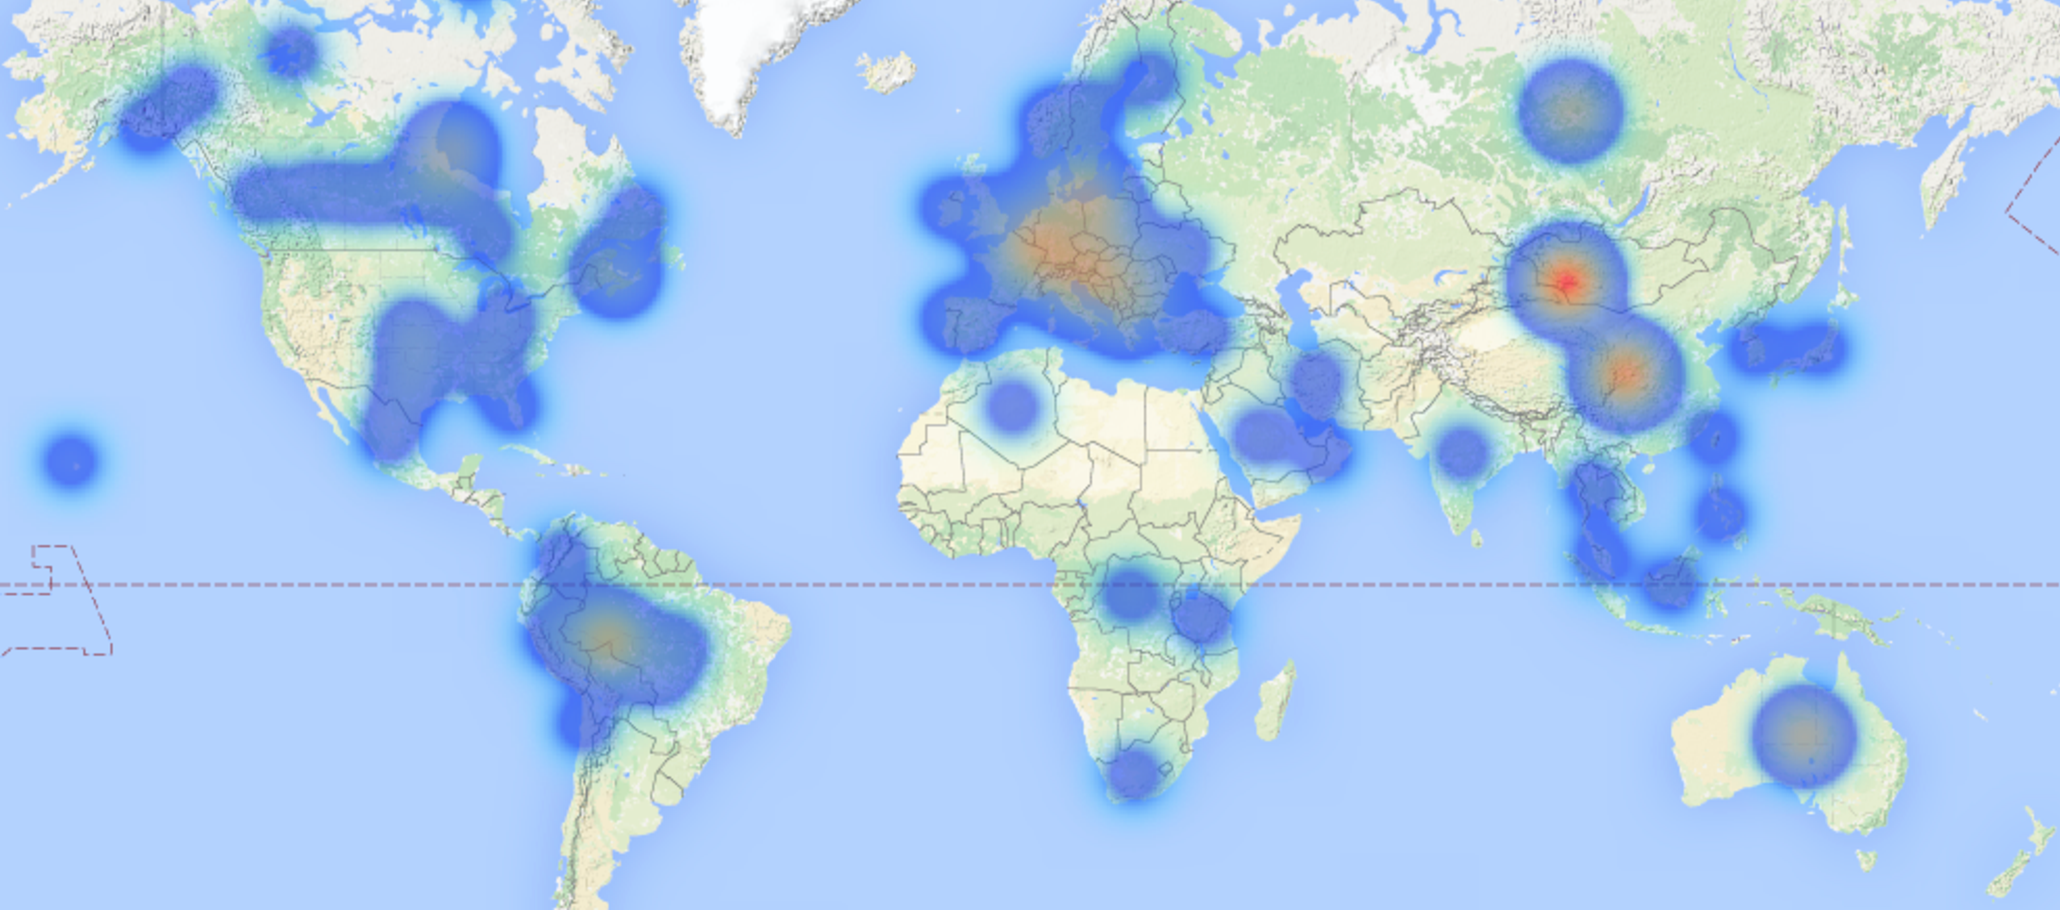
\includegraphics[width=10cm, trim= 0cm 0cm 0cm 0cm,clip]{mapacidification.pdf}
% \caption{Global distribution of terrestrial acidification}
% \label{fig:mapAcid}
% \end{center}
% \end{figure}

\subsection{Sensitivity Analysis}

The the sensitivity analysis is shown in Figure \ref{fig:sens}. The GWP savings from adaptive shading is dependent on the electricity mix as explained in Section \ref{ch:Meth:Opp}. Changing our assumption from the European ENTSO-E mix to a country specific mix brings interesting results. In Switzerland, the mix is dominated by hydro and nuclear power which has a very low GWP potential\cite{itten2012life}. This would then increase the emission factor of the ASF to 70.6 gCO$_{2-eq}$/kWh.
%which is 44\% lower than the emission factor in Switzerland. 
The German mix on the other hand has a higher GWP mix than the ENTSO-E mix due to their high share in coal fire plants. This then reduces the emission factor of the ASF to -792.9 gCO$_{2-eq}$/kWh. This difference arises as the greenhouse gas emission savings of adaptive shading are dependent on the emission factor of the grid mix.\\

We also present a case where we remove the actuators and necessary control system for a dynamic system. Instead we have panels that are optimally orientated at 45$^{\circ}$ to the horizontal axis. This reduces embodied greenhouse gas emissions by 12.1\% from the baseline highlighted in Figure \ref{fig:embodied}. However the reduction in electricity production, and savings through adaptive shading, result in a higher emission factor of -507 gCO$_{2-eq}$/kWh.\\

The choice of actuator has a small impact on the embodied carbon emissions. Changing a single Soft Robotic Actuator (including the air compressor, tubing and maintenance) to a classical servo motor increases the total embodied GWP from 2675.4 kg CO$_{2-eq}$ to 3251.2 kg CO$_{2-eq}$. However, the lower emissions from actuation and maintenance for servo motors cancels out this increase, resulting in an ASF with servo motors having an emission factor of -588.4 gCO$_{2-eq}$/kWh.
%\textcolor{magenta}{\textit{(Is this cited or was it also calculated? Do we provide the inventory?)}} \textcolor{red}{\textit{(Calculated, but inventory of motors needs to go in the Appendix)}}.\\

The control system design should be carefully thought out due to the high embodied GWP of electronic components, these systems contribute to 13\% of total embodied GWP. However limiting the individual actuation of panels to rows does not result in a significant difference. The control system required for an ASF where each panel can be independently actuated has an emission factor of -599.5 gCO$_{2-eq}$/kWh. A system which actuates only rows, has an emission factor of -601.1 gCO$_{2-eq}$/kWh. This 0.3\% difference is insignificant.\\

%\textcolor{red}{The Monte Carlo Simulation did not yield any significant results / was significant. } \textcolor{blue}{Fill this out once your results come in}

% In Switzerland, we see a 6\% reduction compared to the average electricity mix. This is because the Swiss electricity mix is dominated by hydro and nuclear power which has a very low GWP potential [citation needed\textcolor{magenta}{ \textit{ecoinvent?}}]. In Germany on the other hand, the ASF has a 81\% reduction in carbon emissions as the emission factor of the electricity grid is roughly five times higher compared to Switzerland [citation needed] due to the relatively high share in coal-fired power plants.\\

\begin{figure}[H]
\begin{center}
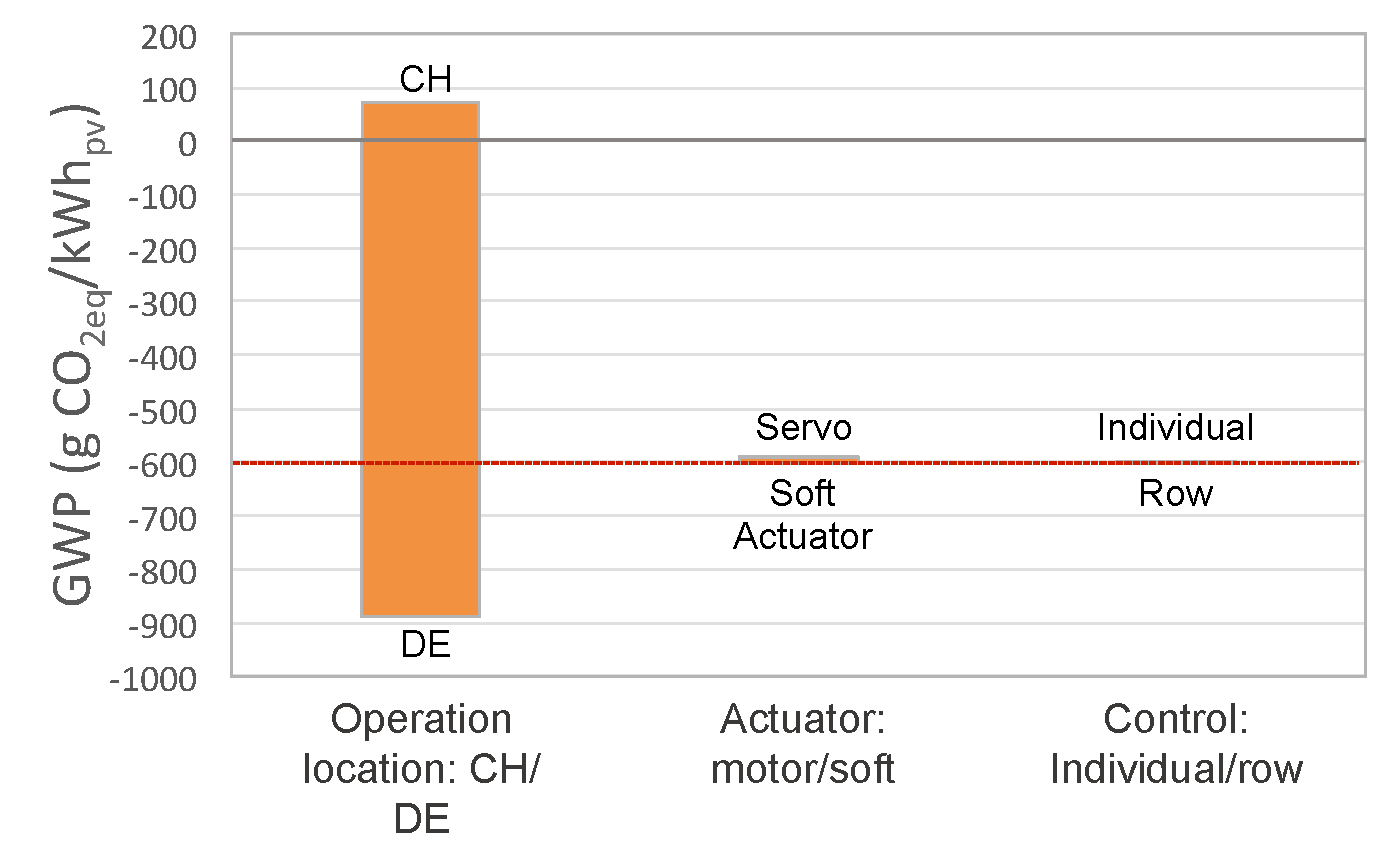
\includegraphics[width=10cm, trim= 0cm 0cm 0cm 0cm,clip]{sens.pdf}
\caption{Sensitivity analysis of the emission factor based on electricity mix, actuation system, and control system}
\label{fig:sens}
\end{center}
\end{figure}

\subsection{Comparison to existing PV technologies}

Comparison of the ASF to other PV technologies and the ENTSO-E electricity mix is highlighted in Figure \ref{fig:compPV}. This comparison is conducted in Switzerland with an average irradiation of 966kWh/m$2$/year.\

The orange bars detail systems with no added shading benefits. Here we present the ASF, a static optimally orientated facade as detailed in Figure \ref{fig:sens}, and three classical flat facade installations.  
The blue bars detail systems built over glazed surfaces which also bring energy savings to the building. Because the GWP savings through adaptive shading offsets the entire embodied GWP, we have a system with a negative emission factor.



%Note that the just panels of the ASF, without the BOS, still has a higher emission factor than the CIGS installation. This is due to lower power production as a result of self shading \cite{hofer2015photovoltaics}, and situations where the panels are not optimally positioned\textcolor{magenta}{\textit{Where do these GHG figures come from?}}.

\begin{figure}[H]
\begin{center}
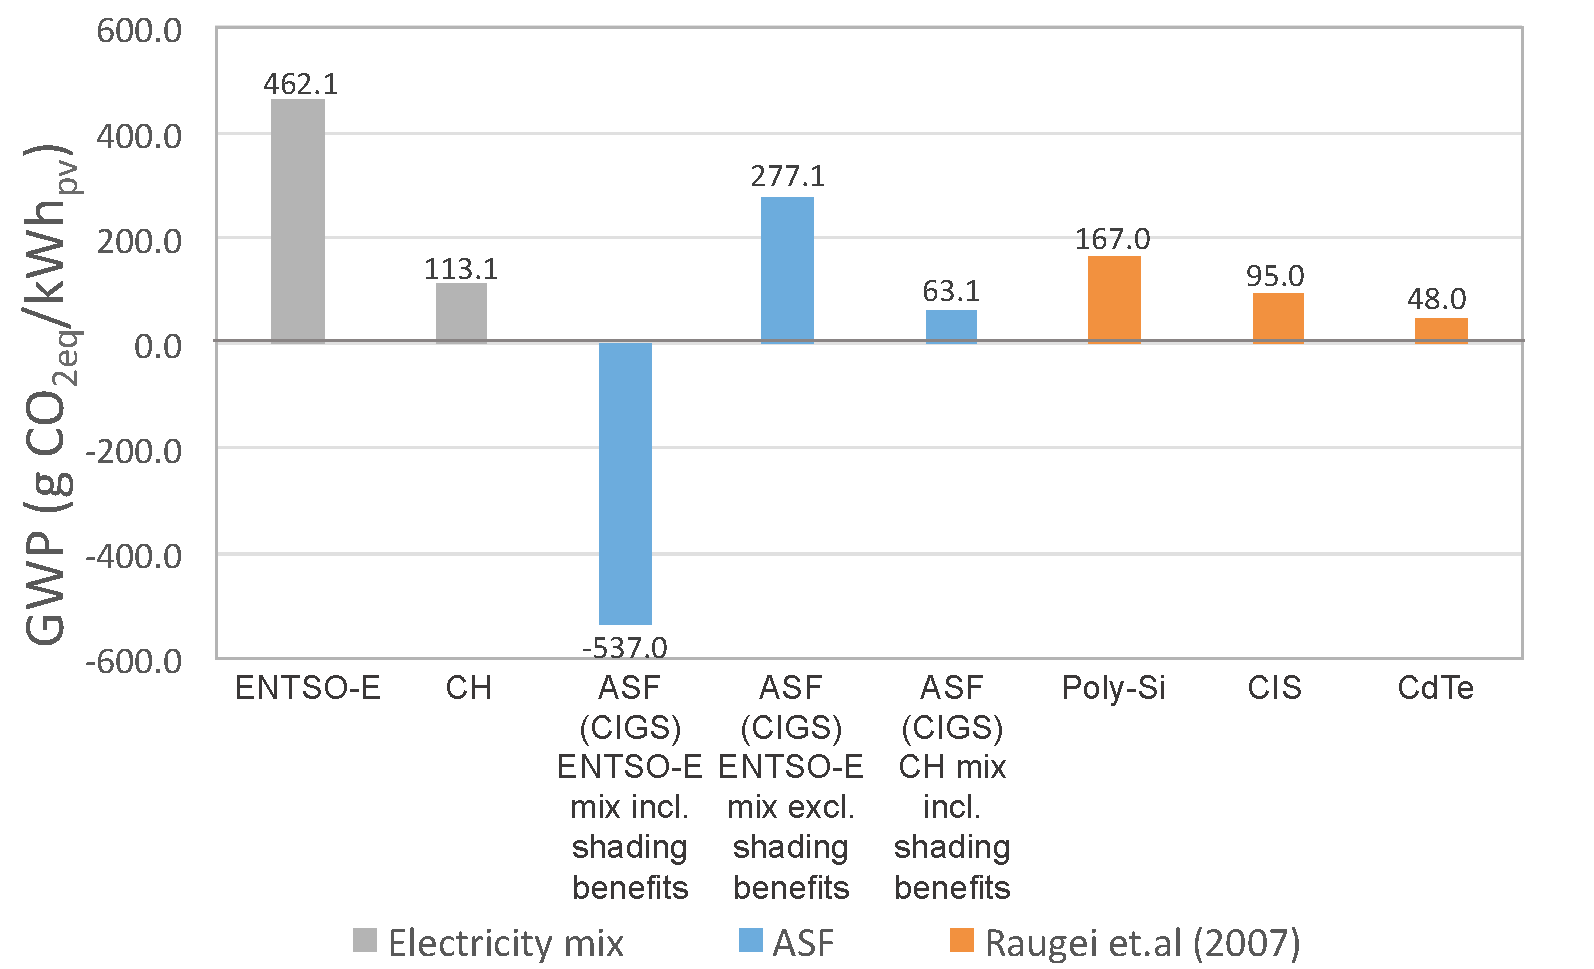
\includegraphics[width=10cm, trim= 0cm 0cm 0cm 0cm,clip]{compPV.pdf}
\caption{Comparison of facade installations in Switzerland with an average irradiation of 966kWh/m2/year.
We compare an ASF to an optimally orientated static facade, and classic flat facade mounted PV solutions. The blue bars include energy savings through shading.}
\label{fig:compPV}
\end{center}
\end{figure}

